
\chapter{Simulation results and agreement}
%general description of results section
This comparative study’s results are organized into four components: (1) the overall statistical metrics for air temperature, specific humidity, and wind speed (i.e., \gls{rmse}, $R^2$, Willmott’s Index of Agreement d, Mean Bias, and \gls{mae}); (2) heatmaps of air temperature, specific humidity, and wind speed from 8 AM–7 PM for both Outdoor+ and ENVI-met; (3) scatter plots for air temperature, specific humidity, and wind speed for both Outdoor+ and ENVI-met; and (4) timeline plots from 8 AM–7 PM for selected locations, including Outdoor+, ENVI-met, and the boundary reference value. This section presents the four components for the Stadium case study in Section 3.1 and Educational Center case study in Section 3.2.

The four comparative components explain the overall agreement between Outdoor+ and ENVI-met under matching conditions for boundary values, vegetation model, and buildings model. Both simulation datasets have equal datapoint length, datapoint location within the simulation domain box, and time window. The overall statistical metrics expose the entire point-to-point dataset agreement. Heatmaps reveal visual patterns and expose the effect of buildings and trees, as well as the gradient distribution for each timestep. Scatter plots illustrate the overall distribution of datapoints where the X-axis represents ENVI-met values as observed values, while the Y-axis represents Outdoor+ values as predicted values. Timeline plots show the simulated values over time and the difference between Outdoor+ results compared to ENVI-met.

%example
\begin{figure}[H]
    \centering
    \includegraphics[width=1\linewidth]{resuls_heatmap_explanation.jpg}
    \caption{Heatmap example, including the case study name, the simulated field, the time, and the wind direction. Sky blue color represents the lowest value in whole simulation, and dark red color represents the highest value.}
    \label{fig:heatmap_explanation}
\end{figure}

\clearpage
\section{Stadium results}
%air temperature, specific humidity, wind speed
%heatmaps
%plots
%statistical metrics
\ref{tab:stadium_stats} shows the statistical metrics for the Stadium case study, tested for air temperature, specific humidity, and wind speed. Air temperature presents a \gls{rmse} value of 2.303, a $R^2$ value of 0.222, a Willmott's Index of Agreement (d) value of 0.65, a Mean Bias value of 0.469, and a \gls{mae} value of 1.393. Specific humidity shows a \gls{rmse} value of 0.003, a $R^2$ value of -12.261, a d value of 0.39, a Mean Bias value of 0.002, and a \gls{mae} value of 0.0027. Wind speed statistical results are 0.877 for \gls{rmse}, -2.884 for $R^2$, 0.415 for d, -0.106 for Mean Bias, and 0.665 for \gls{mae}.

\vspace{0.75cm}

\begin{table}[h!]
    \centering
    \renewcommand{\arraystretch}{1.3}
    \setlength{\tabcolsep}{10pt}
    \caption{Stadium statistical metrics: Root Mean Square Error (RMSE), R Squared ($R^2$), Willmott's Index of Agreement (d), Mean Bias, and Mean Absolute Error (MAE).}
    \resizebox{\textwidth}{!}{
    \begin{tabular}{lrrrrr}
        \toprule
        \textbf{Field} & \textbf{RMSE} & \boldmath$R^2$ & \textbf{d} & 
        \textbf{Mean Bias} & \textbf{MAE}\\
        \midrule
        Temperature & 2.303 & 0.222 & 0.65 & 0.469 & 1.393\\
        Specific humidity & 0.003 & -12.261 & 0.39 & 0.002 & 0.0027\\
        Wind speed & 0.877 & -2.884 & 0.415 & -0.106 & 0.665\\
        \bottomrule
    \end{tabular}
    }
    \label{tab:stadium_stats}
\end{table}



%outdoorplus air temperature table
\begin{figure}
    \centering
    \includegraphics[width=0.9\linewidth]{figures/stadium_temperature_table_2.jpg}
    \caption{Stadium air temperature Outdoor+ simulation results heatmap from 8AM to 7PM.}
    \label{fig:stadium_airtemp_table}
\end{figure}

%envimet air temperature table
\begin{figure}
    \centering
    \includegraphics[width=0.9\linewidth]{figures/envimet_stadium_temperature_table.jpg}
    \caption{Stadium air temperature ENVI-met simulation results heatmap from 8AM to 7PM.}
    \label{fig:stadium_airtemp_table_envimet}
\end{figure}



%statium air temperature scatter plot 
\begin{figure}
    \centering
    \includegraphics[width=1\linewidth]{figures/stadium_-_temperature_scatter_plot_scatter.png}
    \caption{Stadium air temperature scatter plot: observed (ENVI-met) vs. predicted (Outdoor+).}
    \label{fig:stadium_temperature_scatterplot}
\end{figure}



%stadium temperature timeline plots
\begin{figure}
    \centering
    \includegraphics[width=1\linewidth]{figures/stadium_-_temperature_timeline_17406_timeline.png}
    \caption{Stadium air temperature timeline plot for point 17406.}
    \label{fig:stadium_temperature_timeline_17406}
\end{figure}

\begin{figure}
    \centering
    \includegraphics[width=1\linewidth]{figures/stadium_-_temperature_timeline_22026_timeline.png}
    \caption{Stadium air temperature timeline plot for point 22026.}
    \label{fig:stadium_temperature_timeline_22026}
\end{figure}

\begin{figure}
    \centering
    \includegraphics[width=1\linewidth]{figures/stadium_-_temperature_timeline_26383_timeline.png}
    \caption{Stadium air temperature timeline plot for point 26383.}
    \label{fig:stadium_temperature_timeline_26383}
\end{figure}

\begin{figure}
    \centering
    \includegraphics[width=1\linewidth]{figures/stadium_-_temperature_timeline_30395_timeline.png}
    \caption{Stadium air temperature timeline plot for point 30395.}
    \label{fig:stadium_temperature_timeline_30395}
\end{figure}



%outdoorplus humidity table
\begin{figure}
    \centering
    \includegraphics[width=0.9\linewidth]{figures/stadium_humidity_table_2.jpg}
    \caption{Stadium specific humidity Outdoor+ simulation results heatmap from 8AM to 7PM.}
    \label{fig:stadium_humidity_table}
\end{figure}

%envimet humidity table
\begin{figure}
    \centering
    \includegraphics[width=0.9\linewidth]{figures/envimet_stadium_humidity_table.jpg}
    \caption{Stadium specific humidity ENVI-met simulation results heatmap from 8AM to 7PM.}
    \label{fig:stadium_humidity_table_envimet}
\end{figure}



%stadium humidity scatter plot
\begin{figure}
    \centering
    \includegraphics[width=1\linewidth]{figures/stadium_-_humidity_scatter_plot_scatter.png}
    \caption{Stadium specific humidity scatter plot: observed (ENVI-met) vs. predicted (Outdoor+}
    \label{fig:stadium_humidity_scatterplot}
\end{figure}

%stadium humidity timeline plots
\begin{figure}
    \centering
    \includegraphics[width=1\linewidth]{figures/stadium_-_humidity_timeline_17406_timeline.png}
    \caption{Stadium specific humidity timeline plot for point 17406.}
    \label{fig:stadium_humidity_timeline_17406}
\end{figure}

\begin{figure}
    \centering
    \includegraphics[width=1\linewidth]{figures/stadium_-_humidity_timeline_22026_timeline.png}
    \caption{Stadium specific humidity timeline plot for point 22026.}
    \label{fig:stadium_humidity_timeline_22026}
\end{figure}

\begin{figure}
    \centering
    \includegraphics[width=1\linewidth]{figures/stadium_-_humidity_timeline_26383_timeline.png}
    \caption{Stadium specific humidity timeline plot for point 26383.}
    \label{fig:stadium_humidity_timeline_26383}
\end{figure}

\begin{figure}
    \centering
    \includegraphics[width=1\linewidth]{figures/stadium_-_humidity_timeline_30395_timeline.png}
    \caption{Stadium specific humidity timeline plot for point 30395.}
    \label{fig:stadium_humidity_timeline_30395}
\end{figure}



%outdoorplus wind speed table
\begin{figure}
    \centering
    \includegraphics[width=0.9\linewidth]{figures/stadium_windspeed_table_2.jpg}
    \caption{Stadium wind speed Outdoor+ simulation results heatmap from 8AM to 7PM.}
    \label{fig:stadium_windspeed_table}
\end{figure}

%envimet wind speed table
\begin{figure}
    \centering
    \includegraphics[width=0.9\linewidth]{figures/envimet_stadium_windspeed_table.jpg}
    \caption{Stadium wind speed ENVI-met simulation results heatmap from 8AM to 7PM.}
    \label{fig:stadium_windspeed_table_envimet}
\end{figure}



%stadium wind speed scatter plot
\begin{figure}
    \centering
    \includegraphics[width=1\linewidth]{figures/stadium_-_wind_speed_scatter_plot_scatter.png}
    \caption{Stadium wind speed scatter plot: observed (ENVI-met) vs. predicted (Outdoor+}
    \label{fig:stadium_windspeed_scatterplot}
\end{figure}



%stadium wind speed timeline plots
\begin{figure}
    \centering
    \includegraphics[width=1\linewidth]{figures/stadium_-_wind_speed_timeline_17406_timeline.png}
    \caption{Stadium wind speed timeline plot for point 17406.}
    \label{fig:stadium_windspeed_timeline_17406}
\end{figure}

\begin{figure}
    \centering
    \includegraphics[width=1\linewidth]{figures/stadium_-_wind_speed_timeline_22026_timeline.png}
    \caption{Stadium wind speed timeline plot for point 22026.}
    \label{fig:stadium_windspeed_timeline_22026}
\end{figure}

\begin{figure}
    \centering
    \includegraphics[width=1\linewidth]{figures/stadium_-_wind_speed_timeline_26383_timeline.png}
    \caption{Stadium wind speed timeline plot for point 26383.}
    \label{fig:stadium_windspeed_timeline_26383}
\end{figure}

\begin{figure}
    \centering
    \includegraphics[width=1\linewidth]{figures/stadium_-_wind_speed_timeline_30395_timeline.png}
    \caption{Stadium wind speed timeline plot for point 30395.}
    \label{fig:stadium_windspeed_timeline_30395}
\end{figure}


\clearpage
\section{Educational center results}
%air temperature, specific humidity, wind speed
%heatmaps
%plots
%statistical metrics

\begin{figure}[H]
    \centering
    \includegraphics[width=1\linewidth]{figures/Frame_00006_edcenter.png}
    \caption{Educational center air temperature heatmap at 2PM.}
    \label{fig:edcenter_airtemp_2pm}
\end{figure}



\begin{table}[h!]
    \centering
    \renewcommand{\arraystretch}{1.3}
    \setlength{\tabcolsep}{10pt}
    \caption{Educational center statistical metrics: Root Mean Square Error (RMSE), R Squared ($R^2$), Willmott's Index of Agreement (d), Mean Bias, and Mean Absolute Error (MAE).}
    \resizebox{\textwidth}{!}{
    \begin{tabular}{lrrrrr}
        \toprule
        \textbf{Field} & \textbf{RMSE} & \boldmath$R^2$ & \textbf{d} & 
        \textbf{Mean Bias} & \textbf{MAE}\\
        \midrule
        Temperature & 4.625 & -2.187 & 0.192 & 1.143 & 2.959\\
        Specific humidity & 0.003 & -2.49 & 0.33 & 0.001 & 0.002\\
        Wind speed & 0.98 & -3.62 & 0.402 & -0.197 & 0.701\\
        \bottomrule
    \end{tabular}
    }
    \label{tab:edcenter_stats}
\end{table}



%outdoorplus temperature table
\begin{figure}
    \centering
    \includegraphics[width=0.9\linewidth]{figures/edcenter_temperature_table.jpg}
    \caption{Educational center air temperature Outdoor+ simulation results heatmap from 8AM to 7PM.}
    \label{fig:outdoorplus_edcenter_temperature_table}
\end{figure}

%envimet temperature table
\begin{figure}
    \centering
    \includegraphics[width=0.9\linewidth]{figures/envimet_edcenter_temperature_table.jpg}
    \caption{Educational center air temperature ENVI-met simulation results heatmap from 8AM to 7PM.}
    \label{fig:envimet_edcenter_temperature_table}
\end{figure}



%edcenter temperature scatter plot
\begin{figure}
    \centering
    \includegraphics[width=1\linewidth]{figures/educational_center_-_temperature_scatter_plot_scatter.png}
    \caption{Educational center air temperature scatter plot: observed (ENVI-met) vs. predicted (Outdoor+}
    \label{fig:edcenter_temperature_scatterplot}
\end{figure}



%educational center temperature timeline plots
\begin{figure}
    \centering
    \includegraphics[width=1\linewidth]{figures/educational_center_-_temperature_timeline_14089_timeline.png}
    \caption{Educational center air temperature timeline plot for point 14089.}
    \label{fig:edcenter_temperature_timeline_14089}
\end{figure}

\begin{figure}
    \centering
    \includegraphics[width=1\linewidth]{figures/educational_center_-_temperature_timeline_22076_timeline.png}
    \caption{Educational center air temperature timeline plot for point 22076.}
    \label{fig:edcenter_temperature_timeline_22076}
\end{figure}

\begin{figure}
    \centering
    \includegraphics[width=1\linewidth]{figures/educational_center_-_temperature_timeline_27408_timeline.png}
    \caption{Educational center air temperature timeline plot for point 27408.}
    \label{fig:edcenter_temperature_timeline_27408}
\end{figure}

\begin{figure}
    \centering
    \includegraphics[width=1\linewidth]{figures/educational_center_-_temperature_timeline_33635_timeline.png}
    \caption{Educational center air temperature timeline plot for point 33635.}
    \label{fig:edcenter_temperature_timeline_33635}
\end{figure}



%outdoorplus humidity table
\begin{figure}
    \centering
    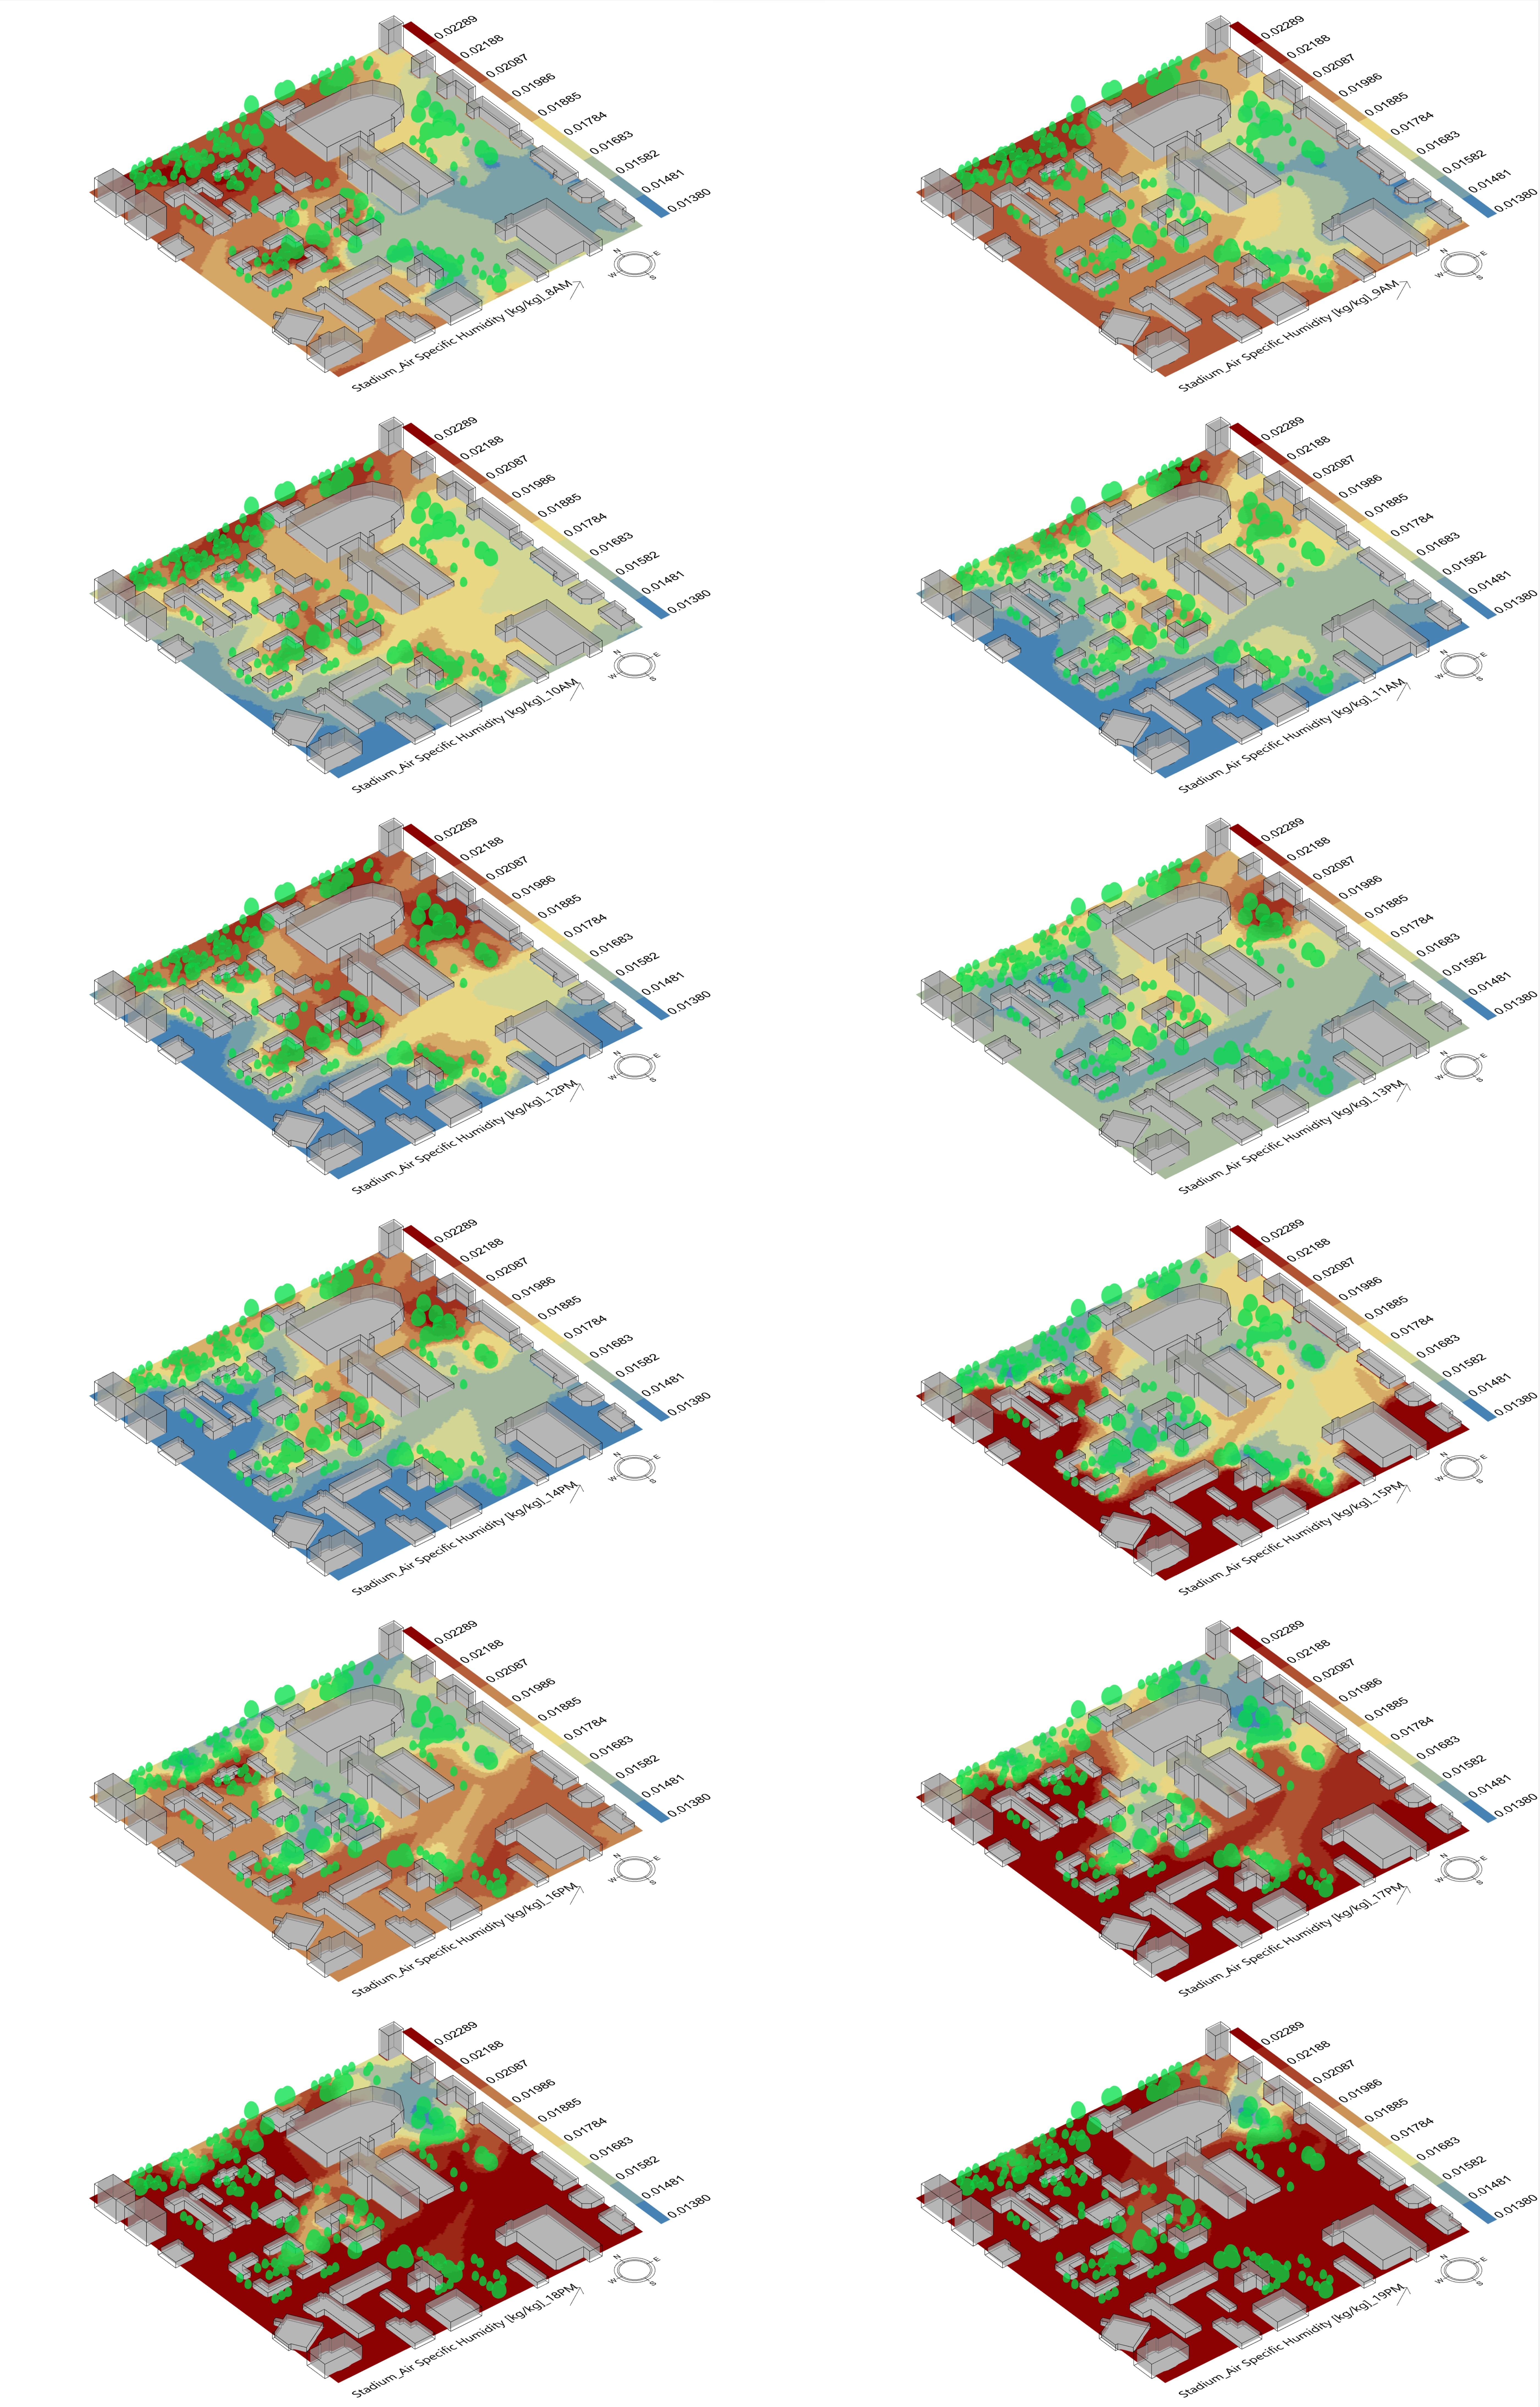
\includegraphics[width=0.9\linewidth]{figures/edcenter_humidity_table.jpg}
    \caption{Educational center specific humidity Outdoor+ simulation results heatmap from 8AM to 7PM.}
    \label{fig:outdoorplus_edcenter_humidity_table}
\end{figure}

%envimet humidity table
\begin{figure}
    \centering
    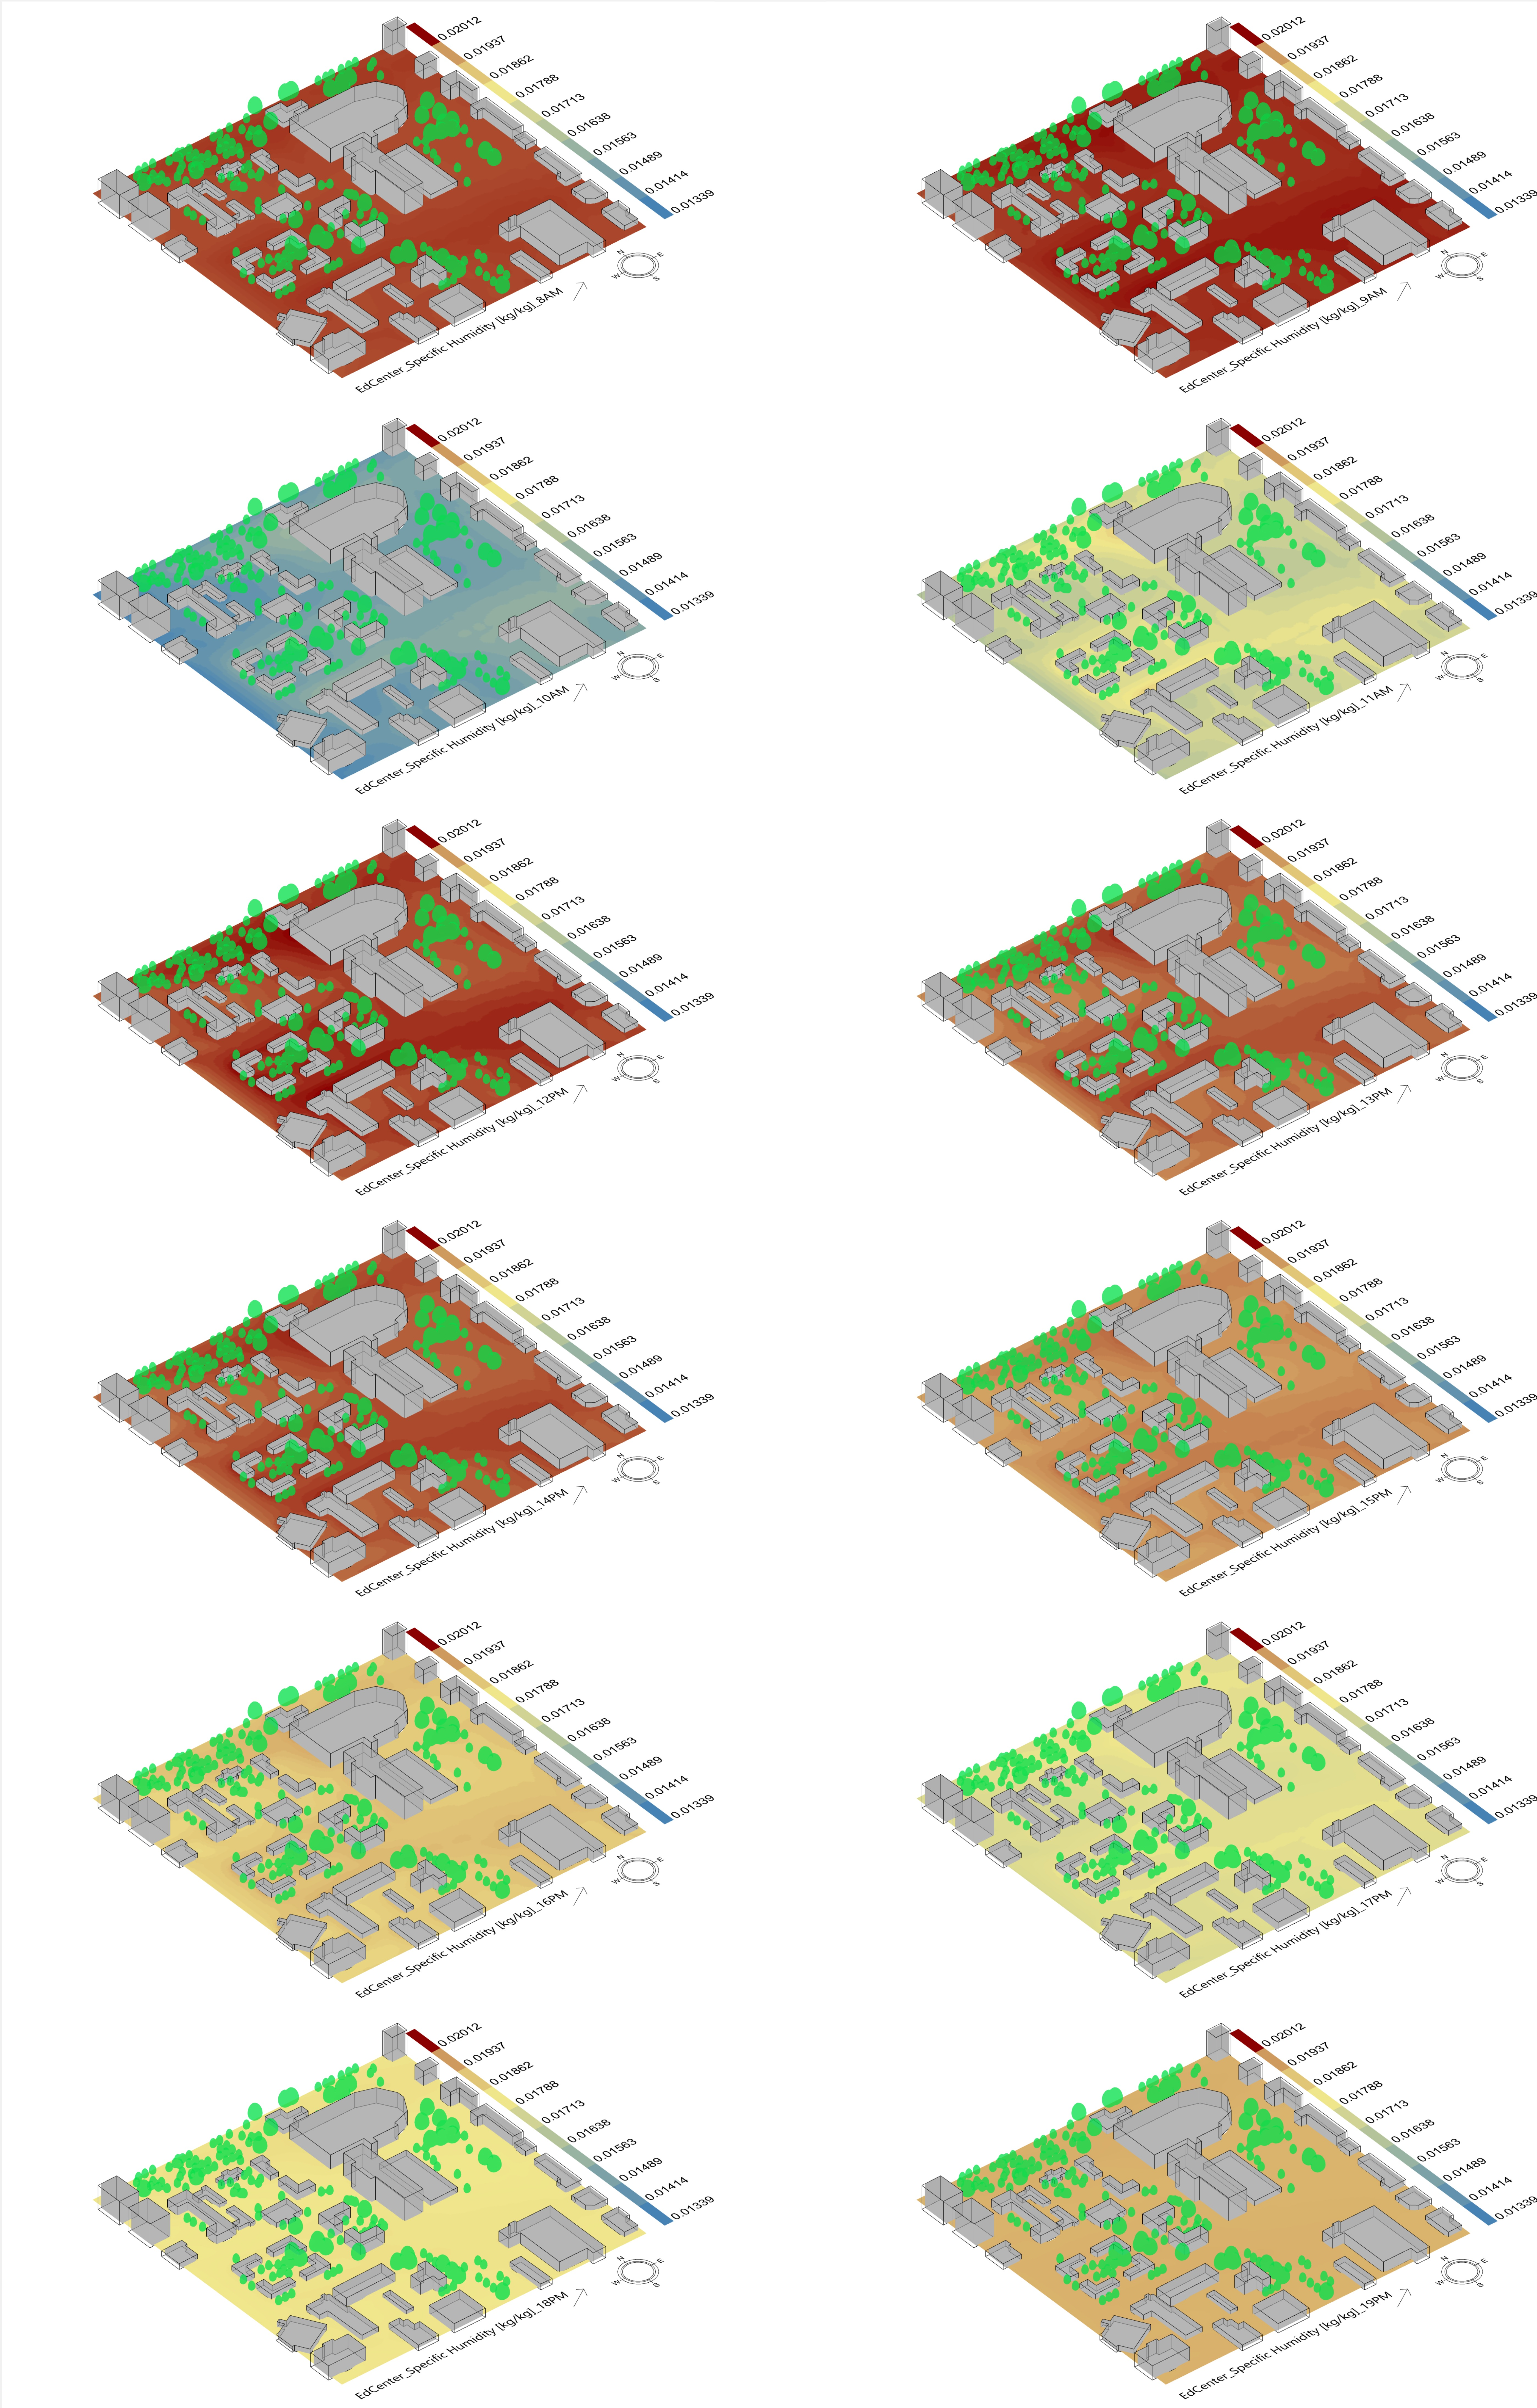
\includegraphics[width=0.9\linewidth]{figures/envimet_edcenter_humidity_table.jpg}
    \caption{Educational center specific humidity ENVI-met simulation results heatmap from 8AM to 7PM.}
    \label{fig:envimet_edcenter_humidity_table}
\end{figure}



%edcenter humidity scatterplot
\begin{figure}
    \centering
    \includegraphics[width=1\linewidth]{figures/educational_center_-_humidity_scatter_plot_scatter.png}
    \caption{Educational center specific humidity scatter plot: observed (ENVI-met) vs. predicted (Outdoor+}
    \label{fig:edcenter_humidity_scatterplot}
\end{figure}



%edcenter humidity timeline plots
\begin{figure}
    \centering
    \includegraphics[width=1\linewidth]{figures/educational_center_-_humidity_timeline_14089_timeline.png}
    \caption{Educational center specific humidity timeline plot for point 14089.}
    \label{fig:edcenter_humidity_timeline_14089}
\end{figure}

\begin{figure}
    \centering
    \includegraphics[width=1\linewidth]{figures/educational_center_-_humidity_timeline_22076_timeline.png}
    \caption{Educational center specific humidity timeline plot for point 22076.}
    \label{fig:edcenter_humidity_timeline_22076}
\end{figure}

\begin{figure}
    \centering
    \includegraphics[width=1\linewidth]{figures/educational_center_-_humidity_timeline_27408_timeline.png}
    \caption{Educational center specific humidity timeline plot for point 27408.}
    \label{fig:edcenter_humidity_timeline_27408}
\end{figure}

\begin{figure}
    \centering
    \includegraphics[width=1\linewidth]{figures/educational_center_-_humidity_timeline_33635_timeline.png}
    \caption{Educational center specific humidity timeline plot for point 33635.}
    \label{fig:edcenter_humidity_timeline_33635}
\end{figure}



%outdoorplus wind speed table
\begin{figure}
    \centering
    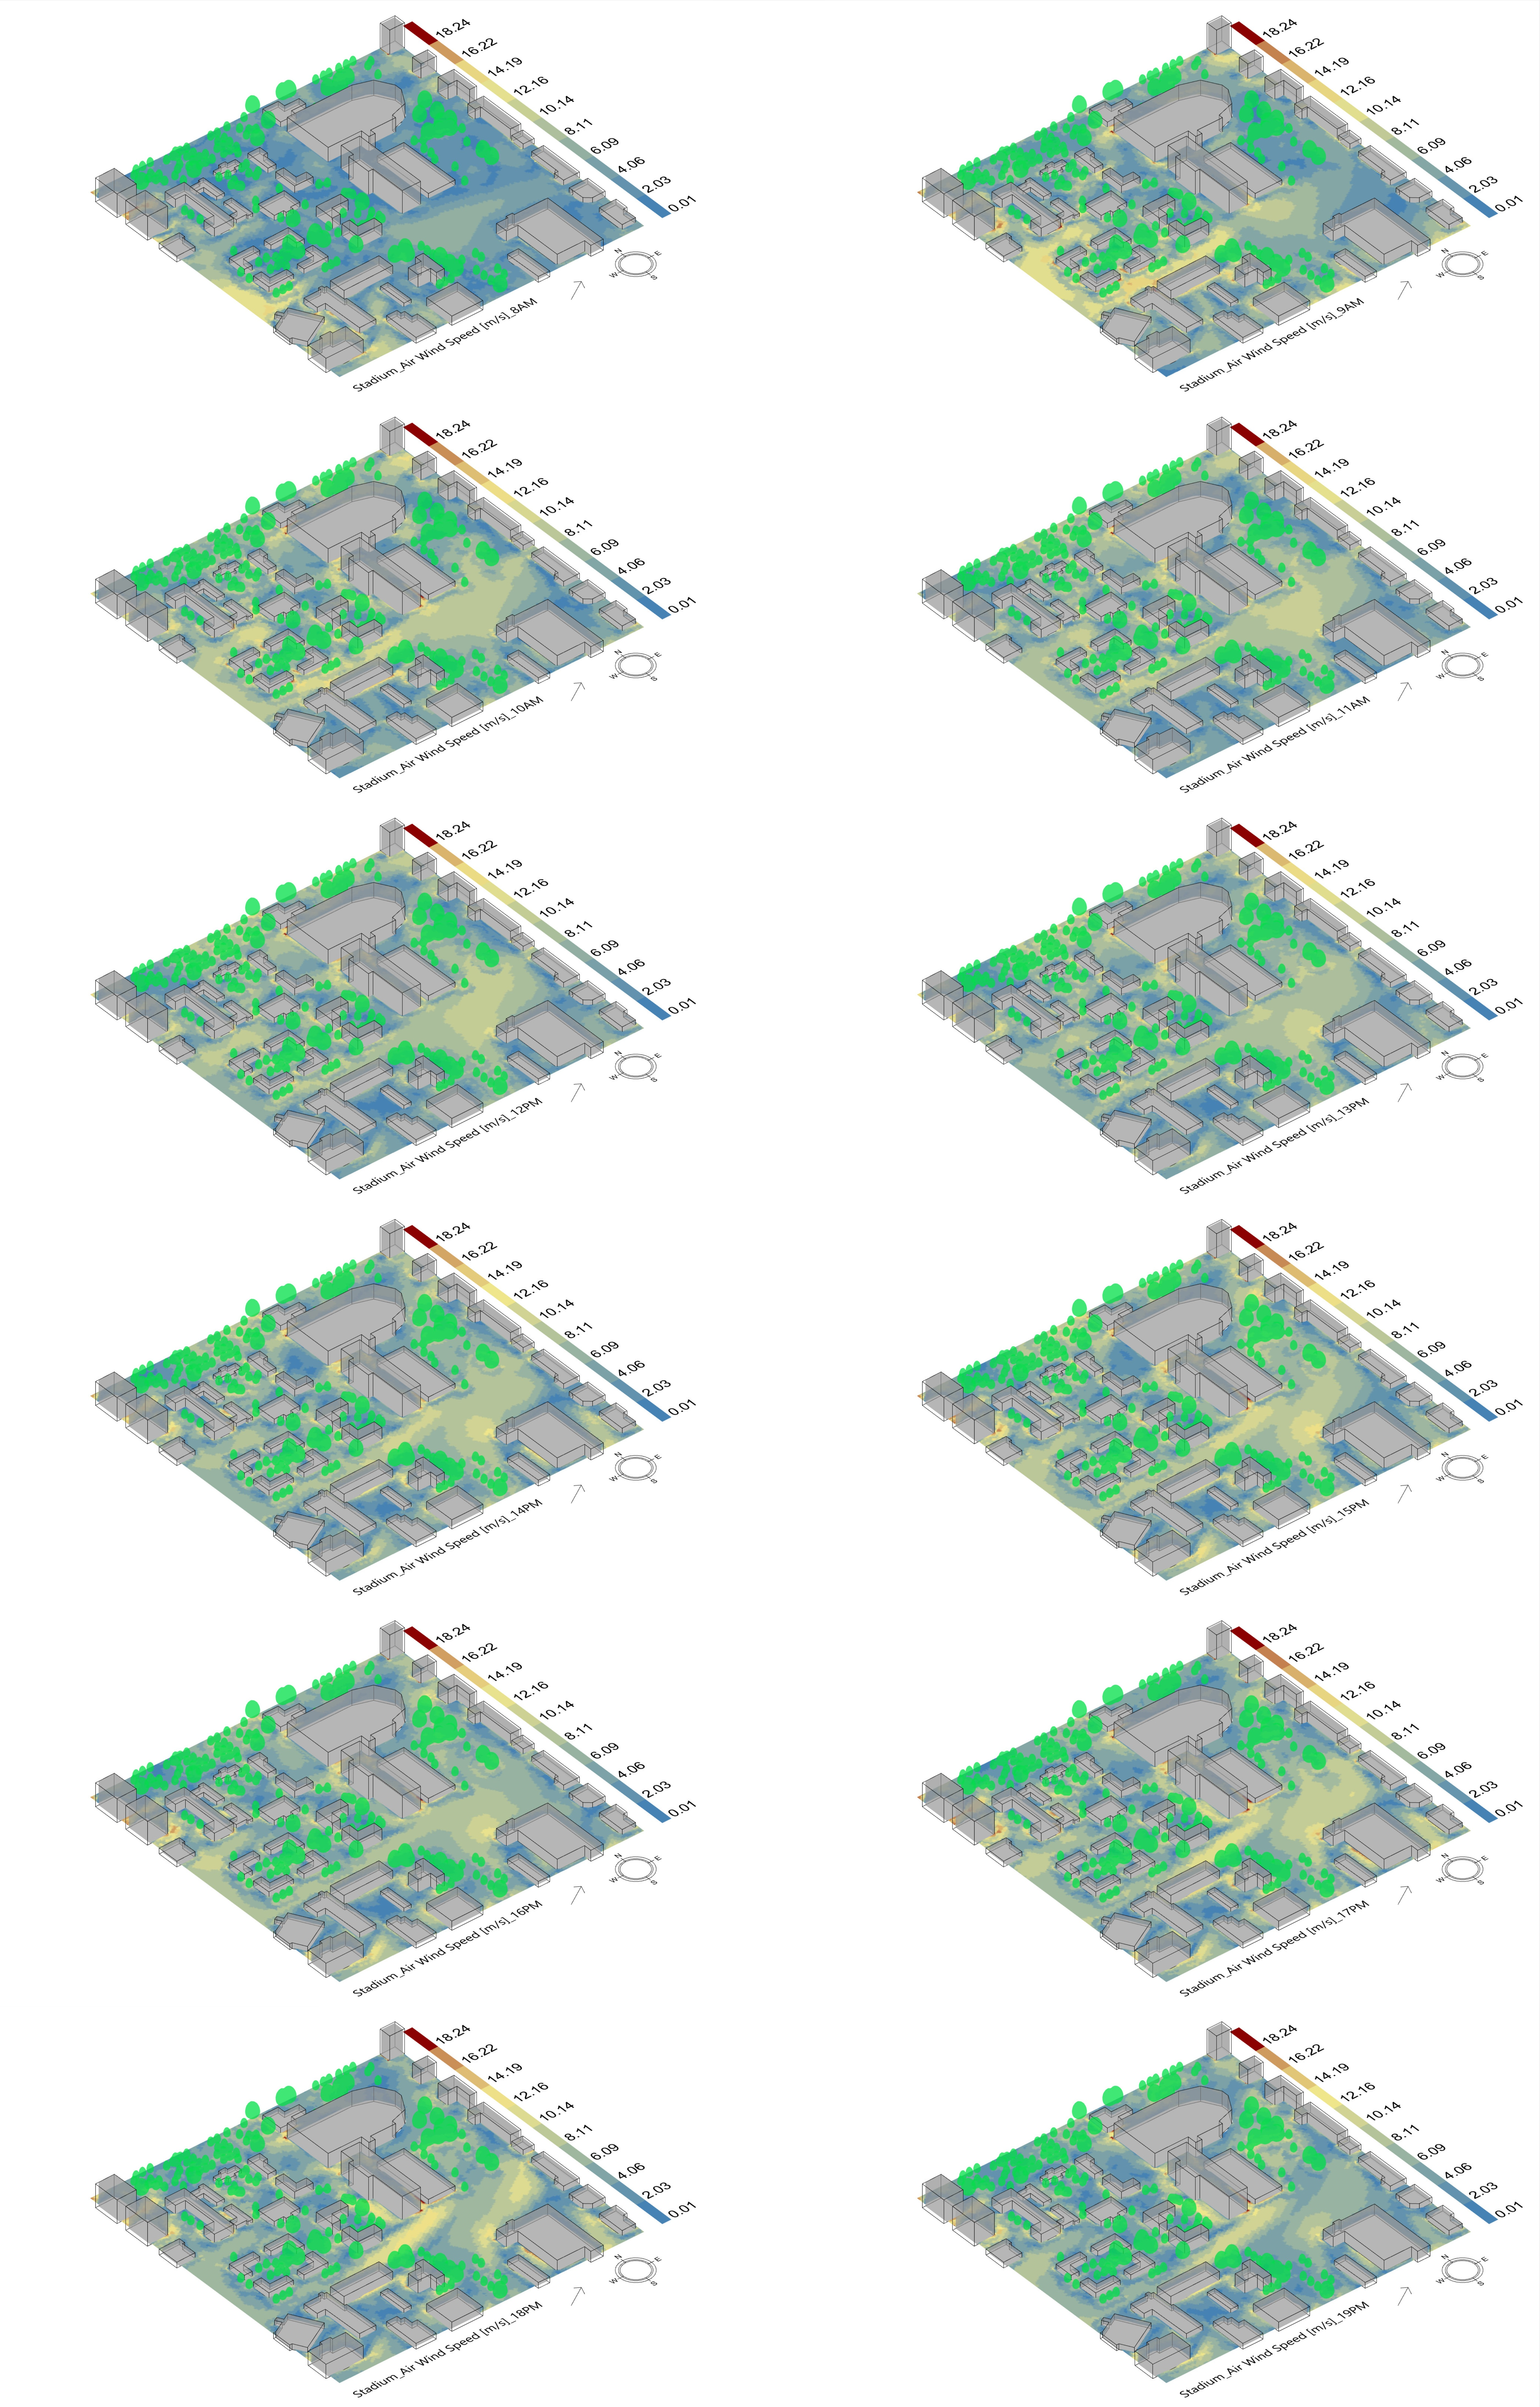
\includegraphics[width=0.9\linewidth]{figures/edcenter_windspeed_table.jpg}
    \caption{Educational center wind speed Outdoor+ simulation results heatmap from 8AM to 7PM.}
    \label{fig:outdoorplus_edcenter_windspeed_table}
\end{figure}

%envimet wind speed table
\begin{figure}
    \centering
    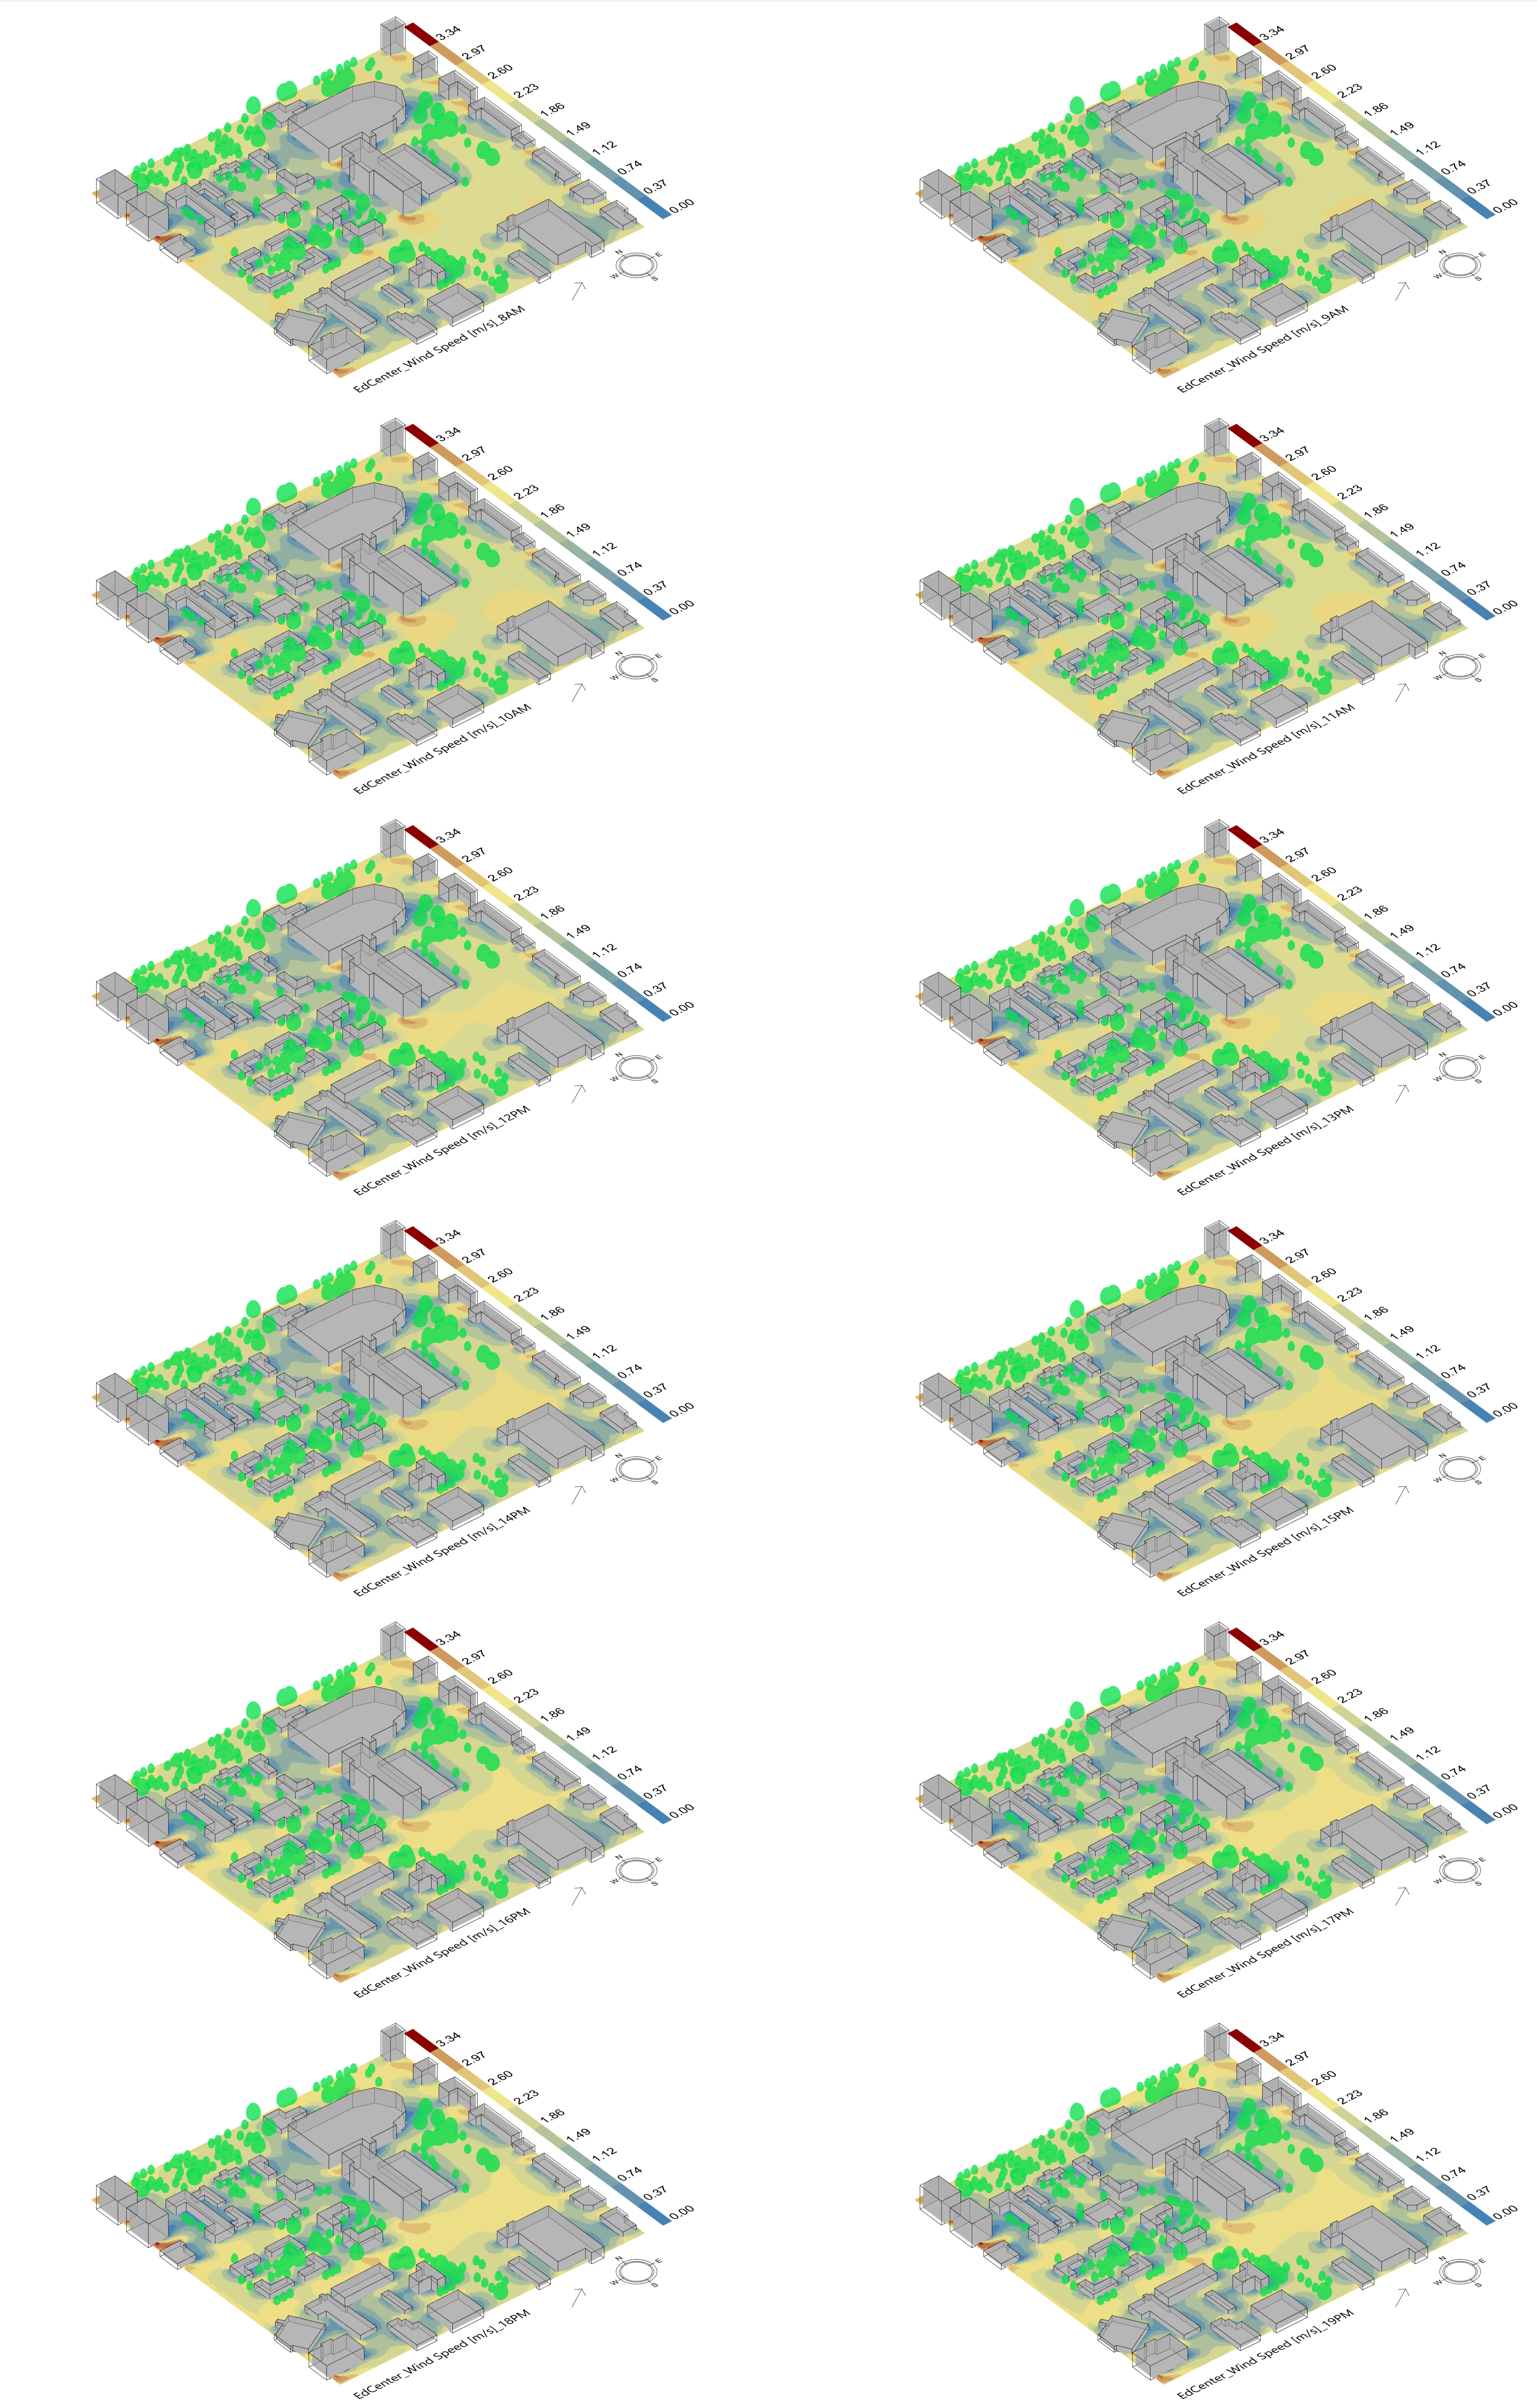
\includegraphics[width=0.9\linewidth]{figures/envimet_edcenter_windspeed_table.jpg}
    \caption{Educational center wind speed ENVI-met simulation results heatmap from 8AM to 7PM.}
    \label{fig:envimet_edcenter_windspeed_table}
\end{figure}



%edcenter wind speed scatter plot
\begin{figure}
    \centering
    \includegraphics[width=1\linewidth]{figures/educational_center_-_wind_speed_scatter_plot_scatter.png}
    \caption{Educational center wind speed scatter plot: observed (ENVI-met) vs. predicted (Outdoor+}
    \label{fig:edcenter_windspeed_scatterplot}
\end{figure}



%edcenter wind speed timeline plots
\begin{figure}
    \centering
    \includegraphics[width=1\linewidth]{figures/educational_center_-_wind_speed_timeline_14089_timeline.png}
    \caption{Educational center wind speed timeline plot for point 14089.}
    \label{fig:edcenter_windspeed_timeline_14089}
\end{figure}

\begin{figure}
    \centering
    \includegraphics[width=1\linewidth]{figures/educational_center_-_wind_speed_timeline_22076_timeline.png}
    \caption{Educational center wind speed timeline plot for point 22076.}
    \label{fig:edcenter_windspeed_timeline_22076}
\end{figure}

\begin{figure}
    \centering
    \includegraphics[width=1\linewidth]{figures/educational_center_-_wind_speed_timeline_27408_timeline.png}
    \caption{Educational center wind speed timeline plot for point 27408.}
    \label{fig:edcenter_windspeed_timeline_27408}
\end{figure}

\begin{figure}
    \centering
    \includegraphics[width=1\linewidth]{figures/educational_center_-_wind_speed_timeline_33635_timeline.png}
    \caption{Educational center wind speed timeline plot for point 33635.}
    \label{fig:edcenter_windspeed_timeline_33635}
\end{figure}